\section{Implementing the editor calculus}

The implementation of the editor calculus requires

\begin{itemize}
\item implementing the semantics of the calculus and allowing for an
  appropriate visualization of editing
\item implementing a type checker based on the type system
\end{itemize}

but perhaps surprisingly, it involves finding a way to script editor
calculus expressions. In this section we outline this.

\subsection{Implementing the editor calculus semantics}

We model the formation rules of the editor calculus by a collection of
algebraic datatypes. As an example, expressions are given by the
datatype

\begin{lstlisting}[language=elm,%
                   label={aep-without-holes-definition},%
                   gobble=4,%
                   caption={Formation rules (\ref{aep-formation-rules}) modeled in Elm},%
                   ]
    type Aep
        = Eval
        | Sub Aam
        | Child Ast.Child
        | Parent
\end{lstlisting}

The rest of the formation rules are defined similarly.

\subsection{Abstract syntax trees}

We are interested in visualizing the AST to make the editor intuitive
for a user.  We are not necessarily interested in finding the ``best''
visualization, nor in implementing a vast number of different
representations.

A simple representation would be to represent the AST in a textual form,
as seen in figure \ref{fig:ast-in-text-form}.

\begin{figure}[H]
    \Large
    \begin{equation*}
      \cursor{(\app{\breakpoint{(\lambda{x}{(\app{x}{x})})}}
      {(\lambda{x}{(\app{x}{x})})})}
    \end{equation*}
    \caption{An AST visualized in textual form.}
    \label{fig:ast-in-text-form}
\end{figure}

The notation used for this representation follows that of Godiksen
et al.~\pepm. It is straightforward but can also be
difficult to reason about, especially as the AST grows large.

We also implement another representatio, namely as a tree as seen in
figure \ref{fig:ast_visual_tree}.

Switching between the two visualizations is immediate in the user interface.

\begin{figure*}
  \center
  \noindent\begin{minipage}{.45\textwidth}
    \center
    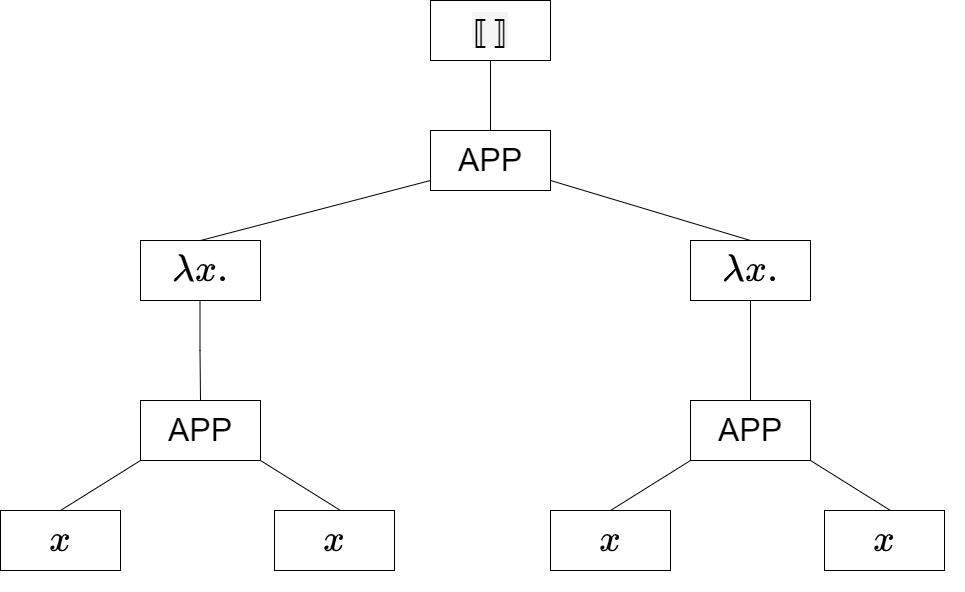
\includegraphics[width=\textwidth]{assets/ast_root_cursor.png}
  \end{minipage}\hfill
  \begin{minipage}{.45\textwidth}
    \center
    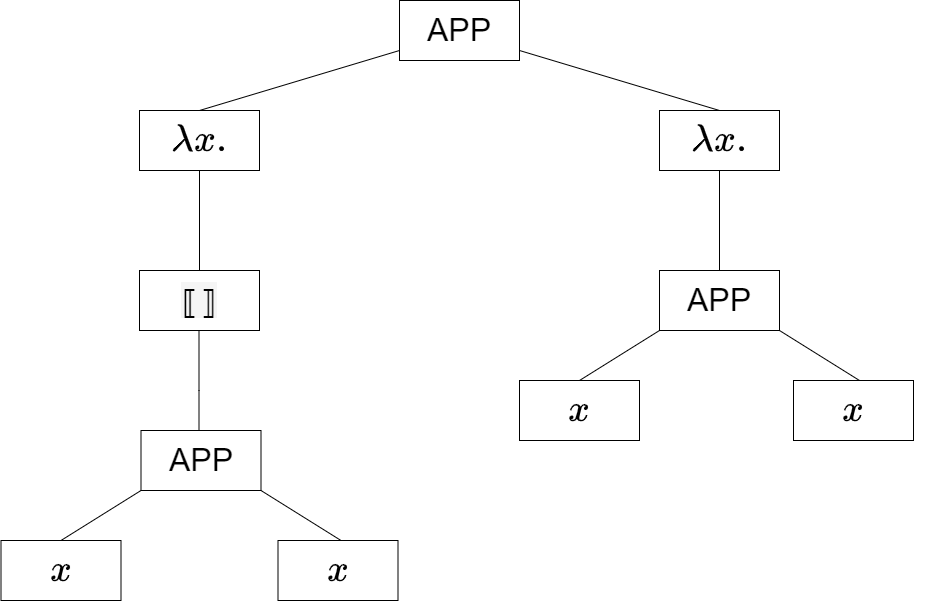
\includegraphics[width=\textwidth]{assets/ast_subtree_cursor.png}
  \end{minipage}\hfill
  \caption{An AST before and after cursor movement visualized in tree form}
  \label{fig:ast_visual_tree}
\end{figure*}

\subsection{Implementing a type checker}


\subsection{Building editor expressions}

To build editor expressions, we need to introduce holes to the editor
expressions. We define a hole term constructor for each type of editor
expression, as seen in figure \ref{fig:editorexpressionswithholes}

\begin{figure}[H]
    \center
    \begin{tabular}{llll}

        \begin{lstlisting}[language=elm,%
                            gobble=8,%
                            mathescape,%
                            ]
             type Aep
                = Eval
                    $\vdots$
                | AepHole
        \end{lstlisting} &

        \begin{lstlisting}[language=elm,%
                            gobble=8,%
                            mathescape,%
                            ]
            type Eed
                = Neg Eed
                     $\vdots$
                | EedHole
        \end{lstlisting} \\

        \begin{lstlisting}[language=elm,%
                            gobble=8,%
                            mathescape,%
                            ]
            type Edt
                = Pre Aep Edt
                    $\vdots$
                | EdtHole
        \end{lstlisting} &

        \begin{lstlisting}[language=elm,%
                            gobble=8,%
                            mathescape,%
                            ]
            type Aam
                = Var Var.Id
                    $\vdots$
                | AamHole
        \end{lstlisting}
    \end{tabular}
    \caption{Editor expression definitions with holes}
    \label{fig:editorexpressionswithholes}
\end{figure}

We are now able to build editor expressions by initializing the editor
expression builder with an \texttt{EdtHole}, and then allow the user to
substitute holes with appropriate expressions. As with ASTs, we have the concept
of atomic editor expressions, which are editor expressions with holes as
children. The user can substitute holes until no holes are left. An editor
expression without any holes is said to be \textit{completed}.

We are only interested in evaluating completed editor expressions. Therefore, we
need to know when an editor expression is completed, and only then allow the
user to evaluate it. To do this, we introduce a type
variable to each editor expression type. The type variable is used
for recursively defining the type in terms of the type variable, but also as an
argument to each hole constructor, as seen in the following listings.

\begin{lstlisting}[language=elm,%
                   label="aep-definition",%
                   gobble=4,%
                   ]
    type Aep a
        = Eval
        | Sub (Aam a)
        | Child Ast.Child
        | Parent
        | AepHole a
\end{lstlisting}

\begin{lstlisting}[language=elm,%
                   label="eed-definitions",%
                   gobble=4,%
                   ]
    type Eed a
        = Neg (Eed a)
        | Conjunction (Eed a) (Eed a)
        | Disjunction (Eed a) (Eed a)
        | At (Aam a)
        | Possibly (Aam a)
        | Necessarily (Aam a)
        | EedHole a
\end{lstlisting}

\begin{lstlisting}[language=elm,%
                   label="generic-edt-definition",%
                   gobble=4,%
                   ]
    type Edt a
        = Pre (Aep a) (Edt a)
        | Bicond (Eed a) (Edt a) (Edt a)
        | SeqComp (Edt a) (Edt a)
        | Rec Var.Id (Edt a)
        | Call Var.Id
        | Nil
        | EdtHole a
\end{lstlisting}

\begin{lstlisting}[language=elm,%
                   label="aam-definitions",%
                   gobble=4,%
                   ]
    type Aam a
        = Var Var.Id
        | Con Const.Value
        | App ATyp ATyp
        | Lambda Var.Id ATyp ATyp
        | Break
        | Hole ATyp
        | AamHole a
\end{lstlisting}

We utilize the \texttt{()} and the \texttt{Never} types to represent
completed and uncompleted editor expressions. If for example \texttt{a} in
\texttt{Edt a} is replaced with \texttt{()}, the editor expression can contain
holes. Conversely, if we replace \texttt{a} with \texttt{Never}, it cannot
contain holes, since we need a \texttt{Never} value to construct a hole. We can
therefore use \texttt{Edt ()} to represent uncompleted editor expressions, and
\texttt{Edt Never} to represent completed editor expressions. We have created a
type alias for completed and uncompleted editor expressions of every type. For
example, the following are the type aliases for \texttt{Edt a}.

\begin{lstlisting}[language=elm,%
                   label="completed-and-uncompleted-edts",%
                   gobble=4,%
                   ]
    type alias Uncompleted =
        Edt ()

    type alias Completed =
        Edt Never
\end{lstlisting}

This approach creates stronger guarantees by making impossible states
impossible. The \texttt{toCompleted} function cannot take an
\texttt{uncompleted} editor expression, return a \texttt{completed} editor
expression and still have bugs, since we have constrained the types to create
type level guarantees.



%%% Local Variables:
%%% mode: latex
%%% TeX-master: "../pepm2023"
%%% End:
